\documentclass[10pt,a4paper,twocolumn]{article}
\usepackage[margin=0.75in]{geometry}
\usepackage{amsmath,amssymb,booktabs,graphicx}
\usepackage{iftex}
\ifPDFTeX
  \usepackage[T1]{fontenc}
  \usepackage[utf8]{inputenc}
\else
  \usepackage{fontspec}
\fi
\usepackage{lmodern}
\usepackage{microtype}
\usepackage{caption}
\usepackage{xcolor}
\usepackage{xurl}
\usepackage[unicode,hidelinks]{hyperref}
\captionsetup{font=small,labelfont=bf}
\setlength{\columnsep}{0.25in}
\setlength{\parindent}{1em}
\setlength{\parskip}{0pt}
\setlength{\emergencystretch}{2em}
\setcounter{secnumdepth}{2}
\providecommand{\tightlist}{\setlength{\itemsep}{0pt}\setlength{\parskip}{0pt}}
% definitions for citeproc citations
\NewDocumentCommand\citeproctext{}{}
\NewDocumentCommand\citeproc{mm}{%
  \begingroup\def\citeproctext{#2}\cite{#1}\endgroup}
\makeatletter
 % allow citations to break across lines
 \let\@cite@ofmt\@firstofone
 % avoid brackets around text for \cite:
 \def\@biblabel#1{}
 \def\@cite#1#2{{#1\if@tempswa , #2\fi}}
\makeatother
\newlength{\cslhangindent}
\setlength{\cslhangindent}{1.5em}
\newlength{\csllabelwidth}
\setlength{\csllabelwidth}{3em}
\newenvironment{CSLReferences}[2] % #1 hanging-indent, #2 entry-spacing
 {\begin{list}{}{%
  \setlength{\itemindent}{0pt}
  \setlength{\leftmargin}{0pt}
  \setlength{\parsep}{0pt}
  % turn on hanging indent if param 1 is 1
  \ifodd #1
   \setlength{\leftmargin}{\cslhangindent}
   \setlength{\itemindent}{-1\cslhangindent}
  \fi
  % set entry spacing
  \setlength{\itemsep}{#2\baselineskip}}}
 {\end{list}}
\usepackage{calc}
\newcommand{\CSLBlock}[1]{\hfill\break\parbox[t]{\linewidth}{\strut\ignorespaces#1\strut}}
\newcommand{\CSLLeftMargin}[1]{\parbox[t]{\csllabelwidth}{\strut#1\strut}}
\newcommand{\CSLRightInline}[1]{\parbox[t]{\linewidth - \csllabelwidth}{\strut#1\strut}}
\newcommand{\CSLIndent}[1]{\hspace{\cslhangindent}#1}

\hypersetup{pdftitle={pygarble: Modular, Low-Cost Gibberish Detection
and Text Screening in Python},pdfauthor={Ujjwal Singh Rao}}
\begin{document}
\raggedbottom
\twocolumn[{
\begin{center}
{\LARGE\bfseries pygarble: Modular, Low-Cost Gibberish Detection and
Text Screening in Python\par}
\vspace{1em}
{\large Ujjwal Singh Rao\par}
\end{center}
\vspace{0.5em}
\begin{center}
\begin{minipage}{0.96\textwidth}
\small\textbf{Abstract.} pygarble is a Python library for inexpensive,
local text screening before downstream processing. Its gibberish module
combines lexical, character statistical and structural signals through a
common interface with configurable thresholds, applicability checks and
inspectable evidence. A separate screening module handles patterns
associated with personal information, secrets and profanity. The base
installation requires neither an inference service nor third-party
runtime dependencies. This paper describes the software architecture and
detection strategies, then evaluates five gibberish configurations
against a pretrained DistilBERT classifier on a complete published
labelled corpus. The 109 source files yield 79,969 common chunks,
including an English comparison of 173 gibberish and 5,200 meaningful
chunks. Word lookup makes no errors on that comparison; the transformer
policy restricted to noise and word salad achieves 99.87\% accuracy with
seven errors. Median single-thread CPU scoring latency is 0.034 ms and
36.369 ms, respectively. The default English ensemble recalls only
28.32\% of gibberish, and other-language diagnostics reveal substantial
false alarms. These results support a configuration-specific, low-cost
screening role on this collection, while exposing limitations of English
lexical assumptions and inherited source labels. The release includes
pinned inputs, predictions and reproducibility checks; performance of
the separate screening module is not evaluated.
\par\vspace{0.5em}
\textbf{Keywords:} text screening; gibberish detection; Python software;
lexical methods; computational efficiency; reproducible evaluation
\end{minipage}
\end{center}
\vspace{1.2em}
}]
\section{Introduction}\label{introduction}

Text-processing pipelines often need to screen inputs before storing,
indexing or analyzing them. Corrupted encodings, keyboard mashing,
invented words and repeated fragments can reduce data quality. Sending
every input to a remote language model introduces an additional service
dependency and inference cost. A local first pass can instead expose
suspicious properties through inexpensive, inspectable rules. Such a
pass must be assessed for both missed defects and false rejection of
meaningful text.

pygarble provides a modular Python implementation of this approach (Rao
2026). Its gibberish detectors combine embedded lexical resources,
character statistics and structural heuristics. Users can select one
strategy or a named ensemble, inspect the contributing signals, and set
a decision policy appropriate to their application. Pattern screening
for personal information, secrets and profanity is isolated in a
separate module because those findings describe different properties
from gibberish. The base library runs without an external inference
service or third-party runtime dependencies.

The software contribution is the integration of these signals into a
reusable interface with explicit applicability, evidence and
configuration; the paper does not propose a new language model or a
general test of meaning. We describe the implementation and evaluate
existing gibberish configurations on a published corpus of
human-produced invented text and meaningful controls. The comparison
with a pretrained DistilBERT classifier measures detection errors and
CPU cost without training either system on the evaluation inputs.

The study addresses three questions: how the library's individual and
ensemble strategies behave on the complete released corpus; how their
detection and false-alarm rates compare with two fixed interpretations
of the neural classifier; and what latency and memory differences arise
on the same local CPU workload. Performance claims are restricted to the
evaluated configurations and data. The separate PII, secret and
profanity facilities are described as software capabilities, without an
empirical accuracy claim in this study.

\section{Background and related work}\label{background-and-related-work}

Lexical membership and character-transition models offer inexpensive
evidence of whether text resembles a reference language. Norvig's
published word and character-frequency resources illustrate this class
of methods (Norvig 2009). Renaud's open-source Gibberish-Detector uses
character Markov transitions to identify improbable strings (Renaud,
n.d.). These methods can expose invented words or unusual character
sequences, but unfamiliar vocabulary is not equivalent to meaningless
language. pygarble combines such signals with structural checks and
makes the policy for combining them explicit.

DistilBERT compresses a pretrained transformer through knowledge
distillation (Sanh et al. 2019). Jindal's released AutoNLP classifier
specializes a DistilBERT model to four labels: clean, mild gibberish,
noise and word salad (Jindal, n.d.). It provides a relevant locally
executable neural comparator. A binary screening decision still requires
an explicit mapping from those four labels, which can materially change
false alarms even when the model probabilities remain fixed.

Gaskell and Bowern study the statistical properties of human-produced
meaningless text in relation to Voynichese (Gaskell and Bowern 2022).
Their accompanying public collection supplies the inherited labels for
this evaluation. It was created for linguistic investigation rather than
sampled from pygarble's intended deployment traffic. The present study
therefore measures performance on an identifiable published collection;
it does not establish general performance on forms, search queries, code
or multilingual user submissions.

\section{Software architecture and detection
strategy}\label{software-architecture-and-detection-strategy}

\subsection{Module boundaries and execution
model}\label{module-boundaries-and-execution-model}

The implementation separates \texttt{pygarble.gibberish} from
\texttt{pygarble.screening}. The former contains
\texttt{GarbleDetector}, \texttt{EnsembleDetector}, strategy
implementations and shared text features. Compatibility exports retain
the existing top-level imports. The latter composes category-specific
detectors for secrets, PII and profanity, with findings and optional
redaction. This separation prevents a PII match from being interpreted
as evidence that a sentence is gibberish.

For gibberish analysis, the detector validates the input and constructs
request-local text features. Cached features include folded text,
tokens, character-bigram statistics and lexical novelty. Tokens preserve
offsets into the original input and identify structured forms such as
URLs or identifiers. Allowlisted tokens can be excluded from
contributing evidence. Strategies share applicable features during
ensemble analysis, while strategy-specific normalization and eligibility
rules remain explicit.

Each strategy returns a score, an applicability flag and a reason, with
matched spans where available. The public analysis result records the
combined decision and individual signals. Scores are heuristic values in
\([0,1]\), not calibrated probabilities, despite the compatibility
method name \texttt{predict\_proba}. An inapplicable strategy does not
vote. When no strategy is applicable, the analysis reports insufficient
evidence and returns an unflagged decision; this status must not be
interpreted as proof that the text is meaningful.

\subsection{Lexical screening}\label{lexical-screening}

The \texttt{word\_lookup} strategy measures the fraction of eligible
words absent from an embedded English word set derived from Norvig's
frequency resource (Norvig 2009). It folds diacritics, extracts
Latin-letter runs and, by default, retains words of at least two
letters. For \(n\) retained tokens \(w_i\) and dictionary \(D\), its
default score is

\begin{equation}
\begin{aligned}
s_{\mathrm{lex}}(x)&=\frac{1}{n}\sum_{i=1}^{n}
\mathbf{1}\{\operatorname{lower}(w_i)\notin D\}\,a(w_i),\\
a(w_i)&=\begin{cases}1/2 & \text{if title-cased},\\1 & \text{otherwise}.\end{cases}
\end{aligned}
\end{equation}

The score is zero when \(n=0\). The title-case weight reduces the
contribution of potential names, without providing a named-entity model.
At the default unknown-word setting, the detector flags a score of at
least 0.5. Changing the strategy's unknown-word threshold rescales its
score so that the configured fraction maps to 0.5. No such adjustment is
made in this evaluation. This mechanism is inexpensive but
language-dependent: normal foreign words can be unknown, while nonsense
constructed entirely from dictionary words can appear acceptable. Text
without eligible Latin-letter words can score zero without having been
meaningfully evaluated for linguistic quality.

\subsection{Character-statistical and structural
signals}\label{character-statistical-and-structural-signals}

The Markov strategy evaluates character bigrams over novel tokens after
excluding dictionary-supported or recognized structured tokens. If
\(\ell\) is their mean log transition probability under the embedded
English model, the default score is

\begin{equation}
\begin{aligned}
s_{\mathrm{Markov}}(x)&=\sigma\bigl(2(-3.5-\ell)\bigr),\\
\sigma(z)&=(1+e^{-z})^{-1}.
\end{aligned}
\end{equation}

Low-probability transitions increase the score. Known words or
insufficient novel text can produce zero evidence rather than a large
novelty penalty. The log-likelihood-ratio strategy uses the mean English
log-bigram probability plus \(\log(27)\) as a comparison with a uniform
reference; its default sigmoid midpoint and scale are \(-1.0\) and
\(1.5\). It requires at least three bigrams. These transformations
standardize score ranges without making them calibrated posterior
probabilities.

The word-anomaly strategy operates at token level to limit dilution of a
suspicious token by surrounding prose. Among eligible ASCII tokens of at
least four letters, it counts novel words whose mean log-bigram
probability is below \(-4.6\). If \(b\) of \(m\) eligible tokens meet
that criterion, the default score is \(\min(1,2b/m)\), with insufficient
evidence when \(m=0\). Matched token offsets can be returned as
explanatory spans.

The separate \texttt{entropy\_based} strategy combines an alphabetic
character-entropy component with a clipped mean-bigram improbability
component, with weights 0.4 and 0.6. Its entropy normalization uses a
4.1-bit English reference, capped by the input-length bound; it is not a
semantic classifier. Additional strategies look for encoding damage,
control characters, keyboard adjacency, repeated material, patterns and
local anomalies. These target different failure modes, so their
usefulness depends on the composition of the input collection.

\subsection{Ensemble policies and screening
extension}\label{ensemble-policies-and-screening-extension}

For applicable strategy scores \(s_j(x)\) and threshold \(\tau\), a
strategy votes positive when \(s_j(x)\geq\tau\). Named English profiles
use the \texttt{any} policy:

\begin{equation}
\widehat y(x)=\mathbf{1}\{\max_{j\in A(x)}s_j(x)\geq\tau\},
\end{equation}

where \(A(x)\) is the set of applicable strategies; an empty set yields
no flag. Other supported policies are \texttt{all}, a strict majority of
votes, an average score and a weighted average. Under majority voting,
the returned average score need not cross the threshold when the vote
decision does. The ordinary \texttt{predict} path can short-circuit
\texttt{any} or \texttt{all} decisions, whereas \texttt{analyze}
collects the complete evidence.

The \texttt{legacy} profile combines Markov, log-likelihood-ratio and
word-anomaly signals. The default \texttt{english} profile adds encoding
damage, keyboard adjacency and control characters;
\texttt{english\_extended} further adds patterns, local anomalies and
repetition. Word lookup is available separately and is not part of these
profiles. Thus, the later comparison between word lookup and the
profiles is not an ablation of a component shared by all systems.

In the independent screening module, \texttt{Scanner} combines built-in
category rules and explicitly selected optional backends. Findings
retain category, kind, span, confidence and reason; category and kind
filters determine which findings are retained. Optional adapters include
local secret scanners such as Gitleaks and detect-secrets. Backend
failures raise an error rather than being silently converted into a
clean scan. These engineering facilities extend the library's scope but
are not tested by the gibberish corpus. They require separate
task-specific evaluations before drawing effectiveness claims.

\section{Experimental design}\label{experimental-design}

\subsection{Corpus and inherited
labels}\label{corpus-and-inherited-labels}

The original release consists of \textbf{text files}, which we call
source documents. It does not contain 79,969 independently labelled
classification examples. Gaskell and Bowern collected human-produced
invented-language material to study statistical resemblance to the
Voynich manuscript (Gaskell and Bowern 2022). Their paper describes 42
volunteers and additional author samples; the public archive contains 38
gibberish transcript files. We use all 38 without inferring missing
participant metadata or claiming access to unreleased samples.

The accompanying archive contains 71 meaningful source files spanning 33
language/variant labels. Four are explicitly English: the KJV New
Testament, a modern NET Bible text, a historical Secreta Alberti
transcription and a Wikipedia-derived Voynich article. We use those four
as the target-language negative controls. The other 67 meaningful texts
form a separate language scope diagnostic. We preserve their meaningful
labels rather than calling foreign-language text gibberish. Voynichese
itself has no established binary label and is excluded. Thus, complete
coverage refers to the released \textbf{labelled} collection, pinned at
revision \texttt{d076a7d081f3}; the full revision and archive hashes are
recorded in \texttt{sources.json}.

No new human annotation or label audit was performed. Original source
labels are inherited throughout. The gibberish material carries a
modified MIT notice and citation requirement; comparison texts retain
their separate source terms. We distribute measurements and retrieval
instructions, not the comparison prose.

\subsection{Common preprocessing}\label{common-preprocessing}

We collapse whitespace, then split each complete source file into
consecutive, nonoverlapping chunks of 400 Unicode characters, retaining
the final shorter chunk. This is \textbf{our preprocessing}, not an
original dataset partition. Each chunk inherits its source file's
meaningful/gibberish label; individual chunks were not separately
annotated by the original authors. Both systems receive exactly the same
text, including fragments that end within a word.

\begin{table}[htbp]
\centering
\small
\caption{Source files and derived chunks in the complete labelled release.}
\begin{tabular}{@{}lrr@{}}
\toprule
Source group & Files & Chunks \\
\midrule
Gibberish & 38 & 173 \\
English controls & 4 & 5,200 \\
Other languages & 67 & 74,596 \\
Total & 109 & 79,969 \\
\bottomrule
\end{tabular}
\end{table}

All 31,964,664 normalized characters are covered. There are 109 short
tails, 0 exact duplicate chunk occurrences and no silently truncated
inputs. The English comparison therefore has \textbf{5,373 chunks},
while the separate language diagnostic contains the remaining 74,596.
The larger total does not mean 79,969 independent observations: chunks
share source files, and several meaningful files are related Bible
translations.

An earlier capped experiment used 38 positive prefixes and 400 English
control blocks. All 438 primary input hashes recur here. The full run
extends coverage; it is not an independent confirmation of the
preliminary findings. The extension's code and protocol were frozen in
\texttt{717ceee} before its new predictions, although preliminary
outcomes were already known. It was not an externally preregistered
study.

\subsection{Evaluated configurations and neural
benchmark}\label{evaluated-configurations-and-neural-benchmark}

We evaluate the \texttt{english}, \texttt{english\_extended} and
\texttt{legacy} profiles, plus the individual \texttt{word\_lookup} and
\texttt{entropy\_based} strategies described above, using default
thresholds of 0.5 and one thread. Named ensembles use \texttt{any}
voting. No configuration is trained or tuned on the evaluation corpus.
Scores and applicability status are saved; none of the recorded package
outputs reports insufficient evidence. An always-keep rule provides a
trivial reference without additional inference.

The neural benchmark is Madhur Jindal's AutoNLP gibberish classifier
(Jindal, n.d.), a 66,956,548-parameter DistilBERT sequence classifier
(Sanh et al. 2019). Revision \texttt{76672dd7d357} and every asset hash
are pinned in \texttt{hf\_model.json}; safetensors weights occupy
267,838,720 bytes. The model card declares MIT. Its named training
dataset was inaccessible through the unauthenticated public API, so
fine-tuning overlap cannot be excluded. Model-card validation scores are
not our results.

The model predicts four classes: clean, mild gibberish, noise and word
salad. We fixed two mappings before scoring: \textbf{HF non-clean} flags
every winning class except clean; \textbf{HF noise/salad} flags only
noise or word salad. Both policies use the highest-probability class,
share the same model run and are reported regardless of performance.
Neither thresholding summed probabilities nor selecting a policy after
examining errors is part of this experiment.

Inference uses local verified assets, CPU float32, PyTorch 2.9.0,
Transformers 4.53.3, evaluation mode and no gradients. Exhaustive
scoring uses batches of eight, four intra-op threads, one inter-op
thread and scaled-dot-product attention. Tokenizer parallelism is
disabled. Dynamic padding preserves complete inputs; the largest
observed input has 348 tokens, below the 512-token limit. The neural
dependencies belong to the research harness, not pygarble's base
installation.

\subsection{Evaluation metrics}\label{evaluation-metrics}

Gibberish is the positive class. A true positive (TP) is a correctly
flagged gibberish chunk, and a false negative (FN) is a missed gibberish
chunk. A false positive (FP) is meaningful text incorrectly flagged, and
a true negative (TN) is meaningful text correctly retained. For \(N\)
evaluated chunks, we report

\begin{align}
\mathrm{Accuracy} &= \frac{\mathrm{TP}+\mathrm{TN}}{N},\\
\mathrm{Precision} &= \frac{\mathrm{TP}}{\mathrm{TP}+\mathrm{FP}},\\
\mathrm{Recall} &= \frac{\mathrm{TP}}{\mathrm{TP}+\mathrm{FN}},\\
\mathrm{F1} &= \frac{2\mathrm{TP}}{2\mathrm{TP}+\mathrm{FP}+\mathrm{FN}}.
\end{align}

Balanced accuracy is the mean of recall and specificity,
\(\mathrm{TN}/(\mathrm{TN}+\mathrm{FP})\), giving equal weight to the
two classes. Precision is undefined when no chunks are flagged. Because
meaningful chunks outnumber gibberish chunks, accuracy is interpreted
alongside the confusion counts, recall, F1 and the always-keep baseline.

Chunk metrics summarize the observed collection. Chunks from the same
source are dependent, so we do not use their total count as the sample
size for binomial confidence intervals. Appendix A reports the
source-level endpoints specified in the frozen protocol, including
conditional Wilson intervals and a paired source bootstrap. Chunk
summaries were added after scoring; the inputs, labels, thresholds and
predictions remain unchanged. The source aggregation and sensitivity
analyses are reported separately from the chunk classification results.

\section{Results}\label{results}

\subsection{Confusion matrices and
accuracy}\label{confusion-matrices-and-accuracy}

\begin{table*}[htbp]
\centering
\small
\caption{Confusion counts on all 5,373 target-comparison chunks. Every row uses
the same 173 gibberish and 5,200 meaningful English chunks. TP: caught
gibberish; FN: missed gibberish; FP: false alarm; TN: correctly retained
text.}
\begin{tabular}{@{}lrrrr@{}}
\toprule
Method & TP & FN & FP & TN \\
\midrule
English & 49 & 124 & 41 & 5159 \\
Extended & 73 & 100 & 58 & 5142 \\
Legacy & 45 & 128 & 6 & 5194 \\
Word lookup & 173 & 0 & 0 & 5200 \\
Entropy & 0 & 173 & 0 & 5200 \\
HF non-clean & 173 & 0 & 1494 & 3706 \\
HF noise/salad & 172 & 1 & 6 & 5194 \\
Always keep & 0 & 173 & 0 & 5200 \\
\bottomrule
\end{tabular}
\end{table*}

\begin{table*}[htbp]
\centering
\small
\caption{Metrics in percent, computed from Table 2. Always-keep precision is
undefined because it predicts no positives. High accuracy alone is
uninformative here: always keep achieves 96.78\% while detecting no
gibberish and has balanced accuracy of 50\%.}
\begin{tabular}{@{}lrrrrr@{}}
\toprule
Method & Accuracy & Precision & Recall & F1 & Balanced acc. \\
\midrule
English & 96.93 & 54.44 & 28.32 & 37.26 & 63.77 \\
Extended & 97.06 & 55.73 & 42.20 & 48.03 & 70.54 \\
Legacy & 97.51 & 88.24 & 26.01 & 40.18 & 62.95 \\
Word lookup & 100.00 & 100.00 & 100.00 & 100.00 & 100.00 \\
Entropy & 96.78 & -- & 0.00 & 0.00 & 50.00 \\
HF non-clean & 72.19 & 10.38 & 100.00 & 18.80 & 85.63 \\
HF noise/salad & 99.87 & 96.63 & 99.42 & 98.01 & 99.65 \\
Always keep & 96.78 & -- & 0.00 & 0.00 & 50.00 \\
\bottomrule
\end{tabular}
\end{table*}

Word lookup makes no errors on these inputs. HF noise/salad misses one
gibberish chunk and falsely flags six meaningful chunks: seven errors,
99.87\% accuracy and 98.01\% F1. This is close performance on this
collection, not statistical equivalence or evidence of universal 100\%
accuracy for word lookup. Both methods may fail on inputs absent from
this corpus.

The default English and extended profiles detect 28.32\% and 42.20\% of
the gibberish chunks, respectively. Their high accuracy largely reflects
correct decisions on the much larger negative class. These findings
support evaluating configurations individually rather than assuming that
an ensemble outperforms a separately available lexical strategy.

\begin{figure*}[htbp]
\centering
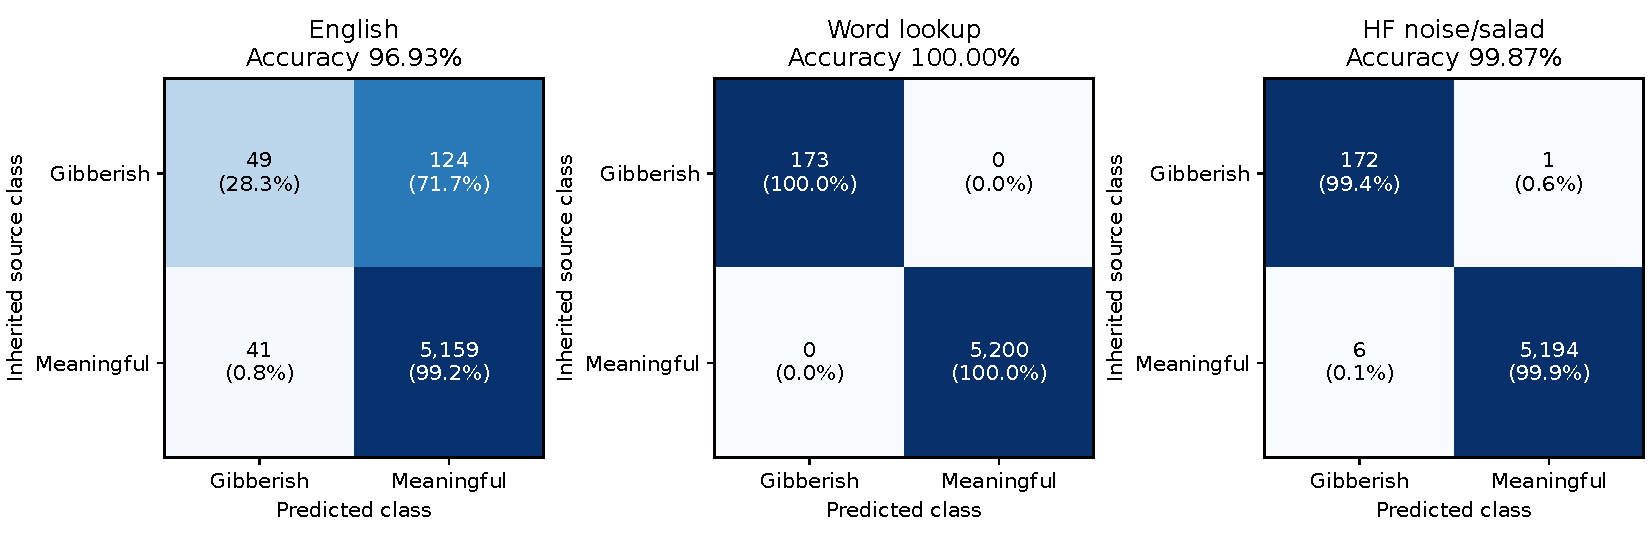
\includegraphics[width=\linewidth]{figures/chunk-confusions.pdf}
\caption{Selected confusion matrices. Cells show counts and within-row
percentages; rows are inherited source labels and columns are predictions.
Row normalization prevents the larger meaningful class from obscuring missed
gibberish. Tables 2--3 report every tested method.}
\label{fig:confusions}
\end{figure*}

\subsection{Label policy and source-specific
errors}\label{label-policy-and-source-specific-errors}

HF non-clean catches all 173 gibberish chunks but falsely flags 1,494
meaningful chunks, producing 72.19\% accuracy and 10.38\% precision.
Exactly 1,488 English control chunks receive the winning label mild
gibberish; these explain the difference from the noise/salad policy. The
policy trade-off therefore concerns how outputs are interpreted, not
different weights or inputs.

\begin{table*}[htbp]
\centering
\small
\caption{False alarms / all chunks in each English source. These source counts
reveal domain differences hidden by a single pooled rate. Precision and
accuracy depend on this study's class balance, not only detector
quality.}
\begin{tabular}{@{}lrrrr@{}}
\toprule
Method & KJV & NET & Wiki & Secreta \\
\midrule
English & 15/2379 & 19/2419 & 2/125 & 5/277 \\
Extended & 22/2379 & 24/2419 & 3/125 & 9/277 \\
Legacy & 4/2379 & 1/2419 & 1/125 & 0/277 \\
Word lookup & 0/2379 & 0/2419 & 0/125 & 0/277 \\
Entropy & 0/2379 & 0/2419 & 0/125 & 0/277 \\
HF non-clean & 579/2379 & 584/2419 & 59/125 & 272/277 \\
HF noise/salad & 5/2379 & 0/2419 & 0/125 & 1/277 \\
\bottomrule
\end{tabular}
\end{table*}

The non-clean policy flags 272 of 277 Secreta chunks, compared with one
for the noise/salad policy. Word lookup has zero observed false alarms
in each control. Four English sources are too few to establish a
population false-positive rate, despite exhaustive coverage within those
sources.

\subsection{CPU and memory
measurements}\label{cpu-and-memory-measurements}

\begin{table}[htbp]
\centering
\small
\caption{Warm CPU scoring latency and separate-worker peak process RSS. The HF
row serves both label policies. Median latency is approximately 1057
times word lookup's and 65.4 times the English profile's on this
workload.}
\begin{tabular}{@{}lrrr@{}}
\toprule
Method & Median ms & p95 ms & RSS (MiB) \\
\midrule
English & 0.556 & 0.673 & 58.5 \\
Extended & 1.048 & 1.199 & 50.5 \\
Legacy & 0.361 & 0.440 & 53.7 \\
Word lookup & 0.034 & 0.040 & 55.0 \\
Entropy & 0.142 & 0.162 & 49.9 \\
HF non-clean & 36.369 & 58.842 & 636.8 \\
\bottomrule
\end{tabular}
\end{table}

Measurements use an Apple M2 with 8 GiB RAM, macOS ARM64 and Python
3.12.2. Each method runs in fresh timing and memory processes after
exhaustive scoring finishes. The fixed workload contains 76 inputs of
400 characters: 38 positive prefixes and 38 deterministically selected
English control blocks. After one warm pass, five measured passes give
380 latency observations per method. Timing uses one thread and batch
size one, including tokenization and model probability work for HF and
the full score/applicability path for pygarble. This differs from the
batched exhaustive run and from a potentially faster short-circuit
\texttt{predict} path. RSS includes the interpreter, imports, model and
resident corpus data. Import, construction, first-call and throughput
data are archived separately.

These are measurements from one CPU and fixed input order, not optimized
neural-runtime comparisons or production latency guarantees. GPU,
quantization, compilation and energy use were not tested. Model download
time is excluded; no paid inference endpoint, data or cloud compute was
procured.

\section{Discussion and limitations}\label{discussion-and-limitations}

The supported finding is narrow but useful: lexical unfamiliarity
separates the released invented texts from these English controls at low
CPU cost. The strict neural policy is also effective. This suggests a
role for simple local screening when invented-word noise resembles the
target data; it does not establish downstream savings in a deployed
pipeline. Ordinary-word semantic nonsense, code, identifiers, names and
real user submissions are not adequately represented here. PII, secrets
and profanity performance was not evaluated.

The other-language diagnostic makes the scope restriction concrete.
Under the study's document rule, word lookup falsely flags 49 of 67
meaningful source files; HF non-clean and HF noise/salad flag 62 and 52.
Appendix B gives all methods and language-level rates. Low false-flag
rates can also be misleading: word lookup returns zero when no eligible
Latin-letter words are found. API-level applicability is not a
certificate of linguistic coverage. Neither system should be presented
as a language-independent test of meaningfulness.

The number of source texts is the central limitation. Many correlated
chunks from four English files do not constitute thousands of
independently collected negative examples. Positive transcripts lack
full participant metadata, source and class are confounded, labels were
inherited without a new audit, and character boundaries can produce
ambiguous fragments. Exact-hash checks found no duplicates, but do not
establish semantic independence or absence of training contamination. HF
fine-tuning overlap and overlap with pre-existing package resources
cannot be ruled out.

The preliminary calibration study remains separately archived. Adapted
character bigram/trigram models following Renaud (Renaud, n.d.) and
package thresholds were calibrated to an empirical 1\% validation
false-positive budget. Transfer failures included 99 false flags in 100
Secreta blocks for a Wiki-calibrated word-lookup threshold and 42\%/44\%
Wiki false-positive rates for the character models. Those are earlier
capped results, not a new full-corpus calibration experiment. They
reinforce the need to validate operating rules on the intended domain.

\section{Reproducibility and
availability}\label{reproducibility-and-availability}

All code, pinned retrieval, asset hashes, predictions, tables, figures
and paper sources are in \texttt{paper/study/} of
\href{https://github.com/brightertiger/pygarble}{the repository}.
\texttt{full-results/} contains this run; \texttt{results/} preserves
the preliminary study. Raw comparison text and model weights remain
outside the repository. Automated checks verify all 79,969 input
identities, coverage and decision mappings and recompute source
summaries. A new offline process replayed 325 fixed inputs from all
documents, with identical decisions and maximum probability difference
of \(1.103\times10^{-6}\). Additional reporting tests independently
reconstruct all target-comparison confusion counts from saved
predictions. The preliminary standard-library experiment has a separate
byte-identical reproduction. These checks validate computations, not
label suitability, and do not constitute independent human or
cross-machine reproduction of the full neural experiment.

\section{Conclusion}\label{conclusion}

pygarble provides a modular local screening library with explicit
strategies, applicability and evidence. Its dictionary strategy is a
competitive and inexpensive option on this published invented-text
collection. The default ensembles, the transformer's label policies and
the other-language diagnostic show why that result must remain
configuration- and domain-specific. The released artifacts make the
trade-off inspectable without adding neural dependencies to the library.

\section*{Declarations}\label{declarations}
\addcontentsline{toc}{section}{Declarations}

\textbf{Funding.} This work received no funding.

\textbf{Competing interests.} The author declares no conflicts of
interest. The author is the developer of pygarble, the software
evaluated in this paper.

\textbf{AI assistance.} OpenAI Codex assisted with study design,
implementation, execution, analysis and manuscript drafting. Anthropic
Claude assisted with coding and running comparison experiments. Exact
model versions were not recorded. No generative LLM supplied evaluation
labels or acted as a judge; DistilBERT is an explicitly evaluated
classifier. Automated checks of the artifacts do not constitute
independent human review of scientific claims.

\onecolumn

\appendix
\setcounter{table}{0}
\setcounter{figure}{0}
\renewcommand{\thetable}{\Alph{section}\arabic{table}}
\renewcommand{\thefigure}{\Alph{section}\arabic{figure}}

\section{Original source-document
endpoints}\label{original-source-document-endpoints}

The frozen protocol specifies a source-file decision that flags a file
when at least half its chunks are flagged, including ties. This is an
evaluation aggregation rather than a native detector operation. The
source-level results are retained alongside the descriptive chunk
summaries added after scoring; \texttt{deviations.md} records the
reporting change. Neither aggregation changes the inherited labels or
detector predictions.

Recall intervals use the Wilson method over 38 positive source files.
Paired recall differences against HF non-clean use 2,000
source-bootstrap replicates with seed 20260926. Both analyses condition
on independent sources; incomplete participant metadata limits that
assumption. Any-chunk decisions and results excluding short tails
provide sensitivity analyses. No equivalence, non-inferiority or
multiple-testing significance claim is made.

\begin{table*}[htbp]
\centering
\small
\caption{TP/FP are source-file decisions; positive/negative means average
within-file flagged fractions with equal file weights. Negative controls
are the four English files. Recall intervals condition on independent
positive files, an assumption limited by incomplete participant
metadata.}
\begin{tabular}{@{}lrrrrr@{}}
\toprule
Method & TP docs & 95\% CI (\%) & Pos. mean & FP docs & Neg. mean \\
\midrule
English & 13/38 & 21.2--50.1 & 34.2\% & 0/4 & 1.21\% \\
Extended & 20/38 & 37.3--67.5 & 47.9\% & 0/4 & 1.89\% \\
Legacy & 13/38 & 21.2--50.1 & 32.1\% & 0/4 & 0.25\% \\
Word lookup & 38/38 & 90.8--100.0 & 100.0\% & 0/4 & 0.00\% \\
Entropy & 0/38 & 0.0--9.2 & 0.0\% & 0/4 & 0.00\% \\
HF non-clean & 38/38 & 90.8--100.0 & 100.0\% & 1/4 & 48.47\% \\
HF noise/salad & 38/38 & 90.8--100.0 & 99.6\% & 0/4 & 0.14\% \\
\bottomrule
\end{tabular}
\end{table*}

\begin{table*}[htbp]
\centering
\small
\caption{Any-chunk source decisions, positive detections after excluding tails
(Full TP), and tail-excluded mean flagged fractions. This provides a
sensitivity check without relabelling or discarding data from the main
run.}
\begin{tabular}{@{}lrrrrr@{}}
\toprule
Method & Any TP & Any FP & Full TP & Full pos. mean & Full neg. mean \\
\midrule
English & 18/38 & 4/4 & 13/38 & 35.9\% & 1.21\% \\
Extended & 26/38 & 4/4 & 18/38 & 48.6\% & 1.90\% \\
Legacy & 15/38 & 3/4 & 13/38 & 33.3\% & 0.25\% \\
Word lookup & 38/38 & 0/4 & 38/38 & 100.0\% & 0.00\% \\
Entropy & 0/38 & 0/4 & 0/38 & 0.0\% & 0.00\% \\
HF non-clean & 38/38 & 4/4 & 38/38 & 100.0\% & 48.37\% \\
HF noise/salad & 38/38 & 2/4 & 38/38 & 100.0\% & 0.14\% \\
\bottomrule
\end{tabular}
\end{table*}

\begin{table}[htbp]
\centering
\small
\caption{Paired source-bootstrap recall differences from HF non-clean, in
percentage points. A zero interval for methods agreeing on every source
reflects this empirical resampling distribution; it is not proof of
equivalent generalization.}
\begin{tabular}{@{}lrr@{}}
\toprule
Method & Delta (pp) & 95\% interval (pp) \\
\midrule
English & -65.8 & -78.9 to -50.0 \\
Extended & -47.4 & -63.2 to -31.6 \\
Legacy & -65.8 & -78.9 to -50.0 \\
Word lookup & 0.0 & 0.0 to 0.0 \\
Entropy & -100.0 & -100.0 to -100.0 \\
HF noise/salad & 0.0 & 0.0 to 0.0 \\
\bottomrule
\end{tabular}
\end{table}

\clearpage

\setcounter{table}{0}
\setcounter{figure}{0}

\section{Other-language scope
diagnostic}\label{other-language-scope-diagnostic}

\begin{table}[htbp]
\centering
\small
\caption{False flags on 67 meaningful source files outside the English controls.
Mean chunk FPR averages source files equally. These negatives remain
separate from the English accuracy and confusion matrices.}
\begin{tabular}{@{}lrr@{}}
\toprule
Method & FP files & Mean FPR \\
\midrule
English & 16/67 & 28.4\% \\
Extended & 18/67 & 32.1\% \\
Legacy & 16/67 & 25.1\% \\
Word lookup & 49/67 & 69.1\% \\
Entropy & 12/67 & 17.9\% \\
HF non-clean & 62/67 & 91.9\% \\
HF noise/salad & 52/67 & 75.8\% \\
\bottomrule
\end{tabular}
\end{table}

\begin{figure*}[htbp]
\centering
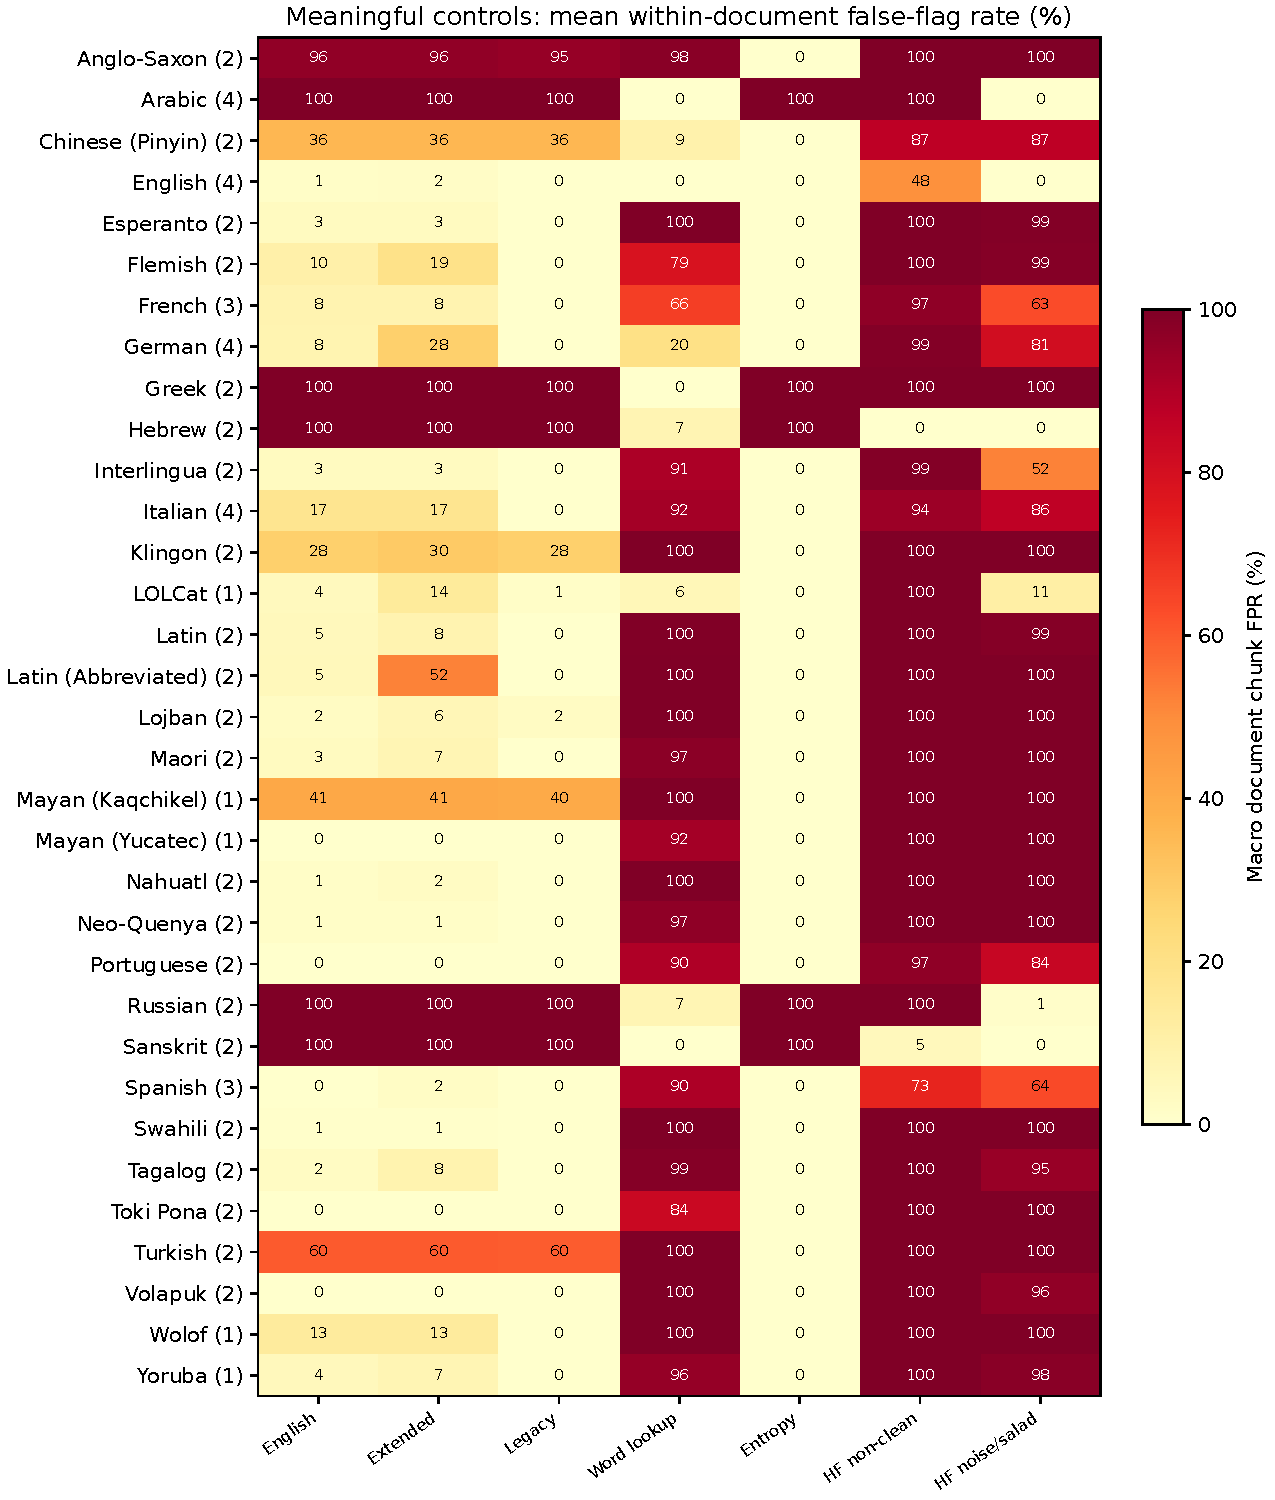
\includegraphics[width=0.65\textwidth]{figures/full-languages.pdf}
\caption{Within-source false-flag rates averaged by supplied language or
variant label. Parentheses give source counts; cells round to whole percentages.
English is included for orientation. Unrounded values are in the released results.}
\label{fig:languages}
\end{figure*}

\twocolumn

\section*{References}\label{references}
\addcontentsline{toc}{section}{References}

\protect\phantomsection\label{refs}
\begin{CSLReferences}{1}{1}
\bibitem[\citeproctext]{ref-gaskell2022}
Gaskell, Daniel E., and Claire L. Bowern. 2022. {``Gibberish After All?
Voynichese Is Statistically Similar to Human-Produced Samples of
Meaningless Text.''} \emph{Proceedings of the International Conference
on the Voynich Manuscript 2022}, CEUR workshop proceedings, vol. 3313.
\url{https://ceur-ws.org/Vol-3313/paper4.pdf}.

\bibitem[\citeproctext]{ref-jindal}
Jindal, Madhur. n.d. \emph{{AutoNLP Gibberish Detector 492513457}}.
Hugging Face. \url{https://doi.org/10.57967/hf/2664}.

\bibitem[\citeproctext]{ref-norvig2009}
Norvig, Peter. 2009. \emph{Natural Language Corpus Data: Beautiful
Data}. \url{https://norvig.com/ngrams/}.

\bibitem[\citeproctext]{ref-pygarble}
Rao, Ujjwal Singh. 2026. \emph{Pygarble: Local Text Screening and
Gibberish Detection}. \url{https://github.com/brightertiger/pygarble}.

\bibitem[\citeproctext]{ref-renaud}
Renaud, Rob. n.d. \emph{{Gibberish-Detector}: A Small Program to Detect
Gibberish Using a {Markov} Chain}.
\url{https://github.com/rrenaud/Gibberish-Detector}.

\bibitem[\citeproctext]{ref-sanh2019}
Sanh, Victor, Lysandre Debut, Julien Chaumond, and Thomas Wolf. 2019.
\emph{{DistilBERT}, a Distilled Version of {BERT}: Smaller, Faster,
Cheaper and Lighter}. \url{https://doi.org/10.48550/arXiv.1910.01108}.

\end{CSLReferences}
\end{document}
